\chapter{Layered Architecture}
\authors{Austin Nicholas Tham, Darren Valentio, Muhammad}



%\gny{Tolong tambahkan keterangan gambar contoh : Gambar 5.1, 5.2, dst.. dan tambahkan italic text untuk setiap bahasa asing}


\section{Definisi \textit{Layered Architechture}}

Pola arsitektur \textit{layered} adalah pola \textit{n-tiered} di mana komponen disusun dalam lapisan horizontal. Ini adalah metode tradisional untuk merancang sebagian besar perangkat lunak dan dimaksudkan untuk pengembangan mandiri sehingga semua komponen saling berhubungan tetapi tidak saling bergantung.

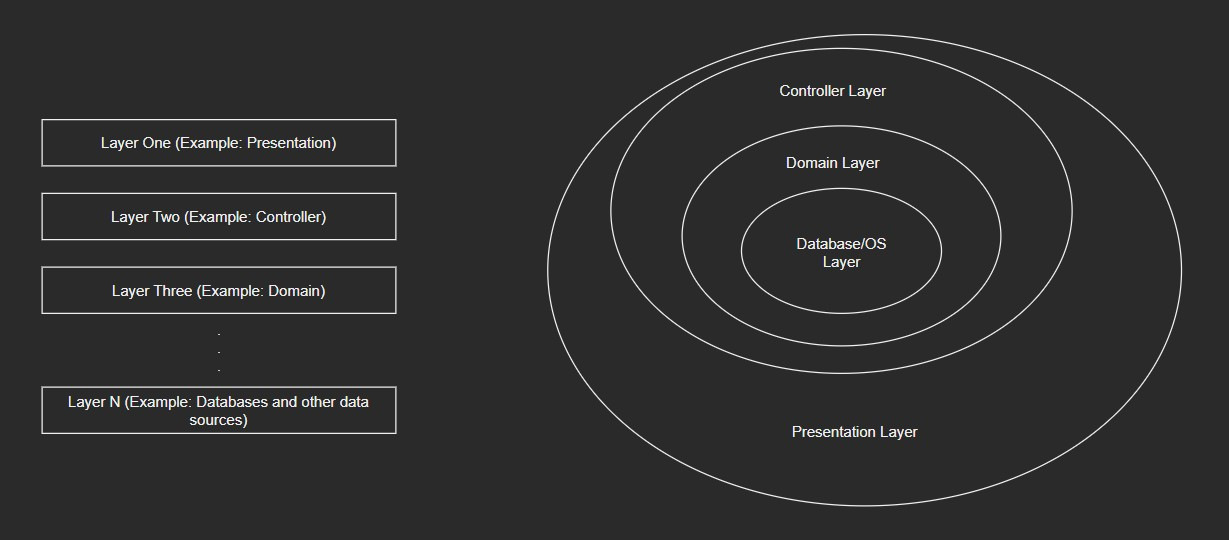
\includegraphics[width=\textwidth]{../images/Layering Architecture}
\begin{center}
	Gambar 5.1 \textit{Layering Architecture}
\end{center}

Seperti yang ditunjukkan pada gambar, \textit{layering} biasanya dilakukan dengan mengemas fungsionalitas khusus aplikasi di lapisan atas, penyebaran fungsionalitas spesifik menjadi lapisan bawah dan fungsionalitas yang membentang di seluruh domain aplikasi di lapisan tengah. Jumlah lapisan dan bagaimana lapisan-lapisan ini disusun ditentukan oleh kompleksitas masalah dan solusinya.

Di sebagian besar arsitektur berlapis, ada beberapa lapisan (atas ke bawah):

\begin{itemize}
    \item \textbf{\textit{The application layered}:} Berisi layanan spesifik aplikasi.
    \item \textbf{The business layer:} Menangkap komponen yang umum di beberapa aplikasi.
    \item \textbf{\textit{The middleware layer}:} Lapisan ini mengemas beberapa fungsi seperti pembangun GUI, antarmuka ke basis data, laporan, dan dll.
    \item \textbf{\textit{The database/System Software Layer}:} Berisi OS, \textit{database}, dan antarmuka ke komponen perangkat keras tertentu.
\end{itemize}

\section{Latar Belakang}

Penilaian untuk setiap karakteristik berdasarkan kecenderungan alami untuk implementasi tipikal pola \textit{layered}.

\begin{itemize}
    \item Kemampuan untuk merespon dengan cepat terhadap lingkungan yang terus berubah. (monolitik)
    \item Bergantung pada implementasi pola, penyebaran bisa menjadi masalah. Satu perubahan kecil ke komponen dapat memerlukan \textit{redeployment} seluruh aplikasi.
    \item Pengembang dapat memberikan pengujian singkat untuk menguji aplikasi sebelum klien menggunakannya
    \item Mudah dikembangkan karena polanya sudah terkenal dan tidak terlalu rumit untuk melakukan implementasinya.
\end{itemize}

\section{Pros Cons}

\subsection{Pros}

\begin{itemize}
    \item Mudah untuk diuji karena komponen-komponennya termasuk lapisan khusus sehingga dapat diuji secara terpisah.
    \item Sederhana dan mudah diimplementasikan karena secara alami, sebagian besar aplikasi bekerja berlapis-lapis
\end{itemize}

\subsection{Cons}

\begin{itemize}
    \item Tidak mudah untuk melakukan perubahan pada lapisan tertentu karena aplikasi merupakan unit tunggal.
    \item Kopling antar lapisan cenderung membuatnya lebih sulit. Hal ini membuatnya sulit untuk diukur.
    \item Harus digunakan sebagai unit tunggal sehingga perubahan ke lapisan tertentu berarti seluruh sistem harus dipekerjakan kembali.
    \item Semakin besar, semakin banyak sumber daya yang dibutuhkan untuk permintaan untuk melewati beberapa lapisan dan dengan demikian akan menyebabkan masalah kinerja.
\end{itemize}

\section{Software Architechture Pattern}
Ini adalah pola arsitektur paling umum di sebagian besar aplikasi tingkat perusahaan. Ini juga dikenal sebagai pola n-tier, dengan asumsi n jumlah tingkatan. Contoh Skenario:

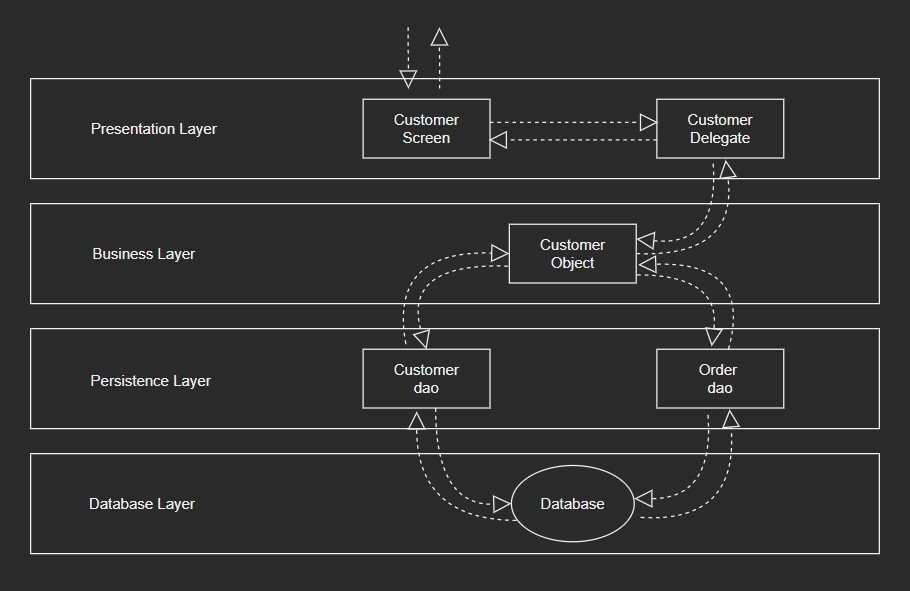
\includegraphics[width=\textwidth]{../images/Software Architecture Pattern}
\begin{center}
	Gambar 5.2 \textit{Software Architecture Pattern}
\end{center}


\section{Design Patterns}

Anggap \textit{mock-up software design}, susunan “\textit{stack}” nya seperti \textit{layered architecture}:

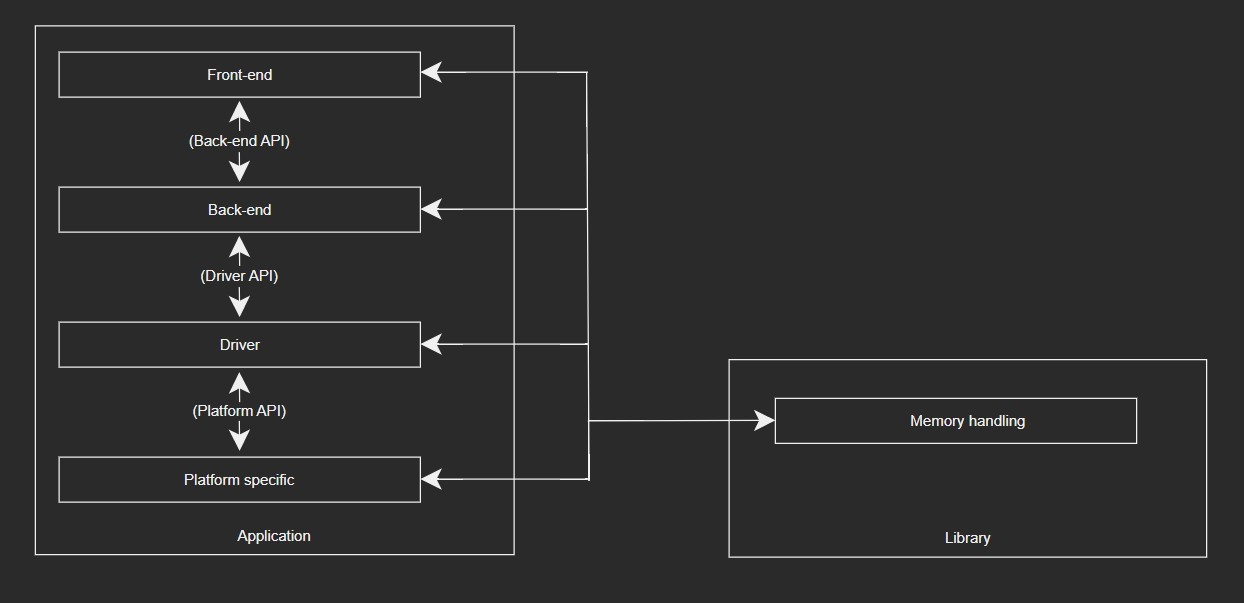
\includegraphics[width=\textwidth]{../images/Design Pattern}
\begin{center}
	Gambar 5.3 \textit{Design Pattern}
\end{center}

Setiap \textit{layer} dari aplikasi terpisah dengan cara penggunaan metode API, namun yang masih saling berhubungan adalah \textit{memory handling} , karena setiap komunikasi \textit{layer} akan membawa/mengirim data sehingga akan terjadi alokasi \textit{memory} dan pada akhirnya membutuhkan \textit{memory handling}.

Ada 4 bagian dari \textit{layered architecture} yang di mana setiap layer memiliki hubungan antara komponen yang ada di dalamnya dari atas ke bawah yaitu:

\begin{itemize}
    \item \textbf{\textit{The presentation layer}:} Semua bagian yang berhubungan dengan layer presentasi.
    \item \textbf{\textit{The business layer}:} Berhubungan dengan logika bisnis.
    \item \textbf{\textit{The persistence layer}:} Berguna untuk mengurusi semua fungsi yang berhubungan dengan objek relasional
    \item \textbf{\textit{The database layer}:} Tempat penyimpanan semua data layer.
\end{itemize}

\subsection{Contoh penerapan \textit{layered architecture}:}

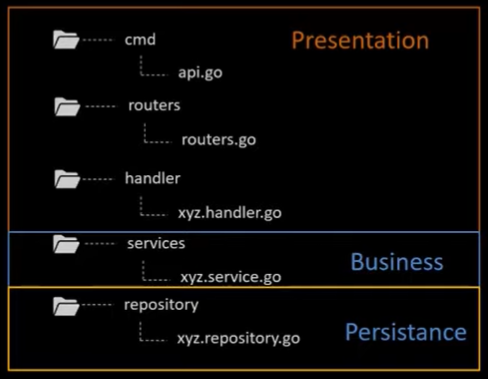
\includegraphics[width=\textwidth]{../images/contoh}
\begin{center}
	Gambar 5.4 Contoh penerapan \textit{layered architecture}
\end{center}

